\documentclass[14pt]{extreport}
  \usepackage[left=1.5cm,right=1.0cm,top=1.5cm,bottom=1.5cm,bindingoffset=0cm]{geometry}
\usepackage[utf8]{inputenc}
\usepackage[english,russian,ukrainian]{babel}
\usepackage{indentfirst}
\usepackage{misccorr}
\usepackage{graphicx}
\usepackage[dvipsnames]{xcolor}
\usepackage{hyperref}
\usepackage{cmap}
\usepackage{amsmath,amsfonts,amssymb,amsthm,mathtools}
\usepackage{icomma}
\usepackage{multirow}
\usepackage{geometry} \geometry{verbose,a4paper,tmargin=1cm,bmargin=2.5 cm,lmargin=2cm,rmargin=1cm}
\usepackage{euscript}
\usepackage{mathrsfs}
\usepackage{mathtext}
\usepackage{graphicx}
\usepackage{booktabs}
\usepackage[normalem]{ulem}
\usepackage{color}
\usepackage{rotating}
\usepackage{pdflscape}
\usepackage{floatrow}
\usepackage{subcaption}
\usepackage{dblfloatfix}
\usepackage{fontawesome5}
\usepackage{calc}
\usepackage{tikz}
\usetikzlibrary{shapes.geometric, arrows}
\usepackage[siunitx]{circuitikz}
\linespread{1.3}
\setlength{\parindent}{5ex}


\begin{document}

\pagecolor{white}
\begin{titlepage}
  \begin{center}
    \large
    Національний технічний університет України \\ "Київський політехнічний інститут імені Ігоря Сікорського"
     
       
    Факультет Електроніки
     
    Кафедра мікроелектроніки
    \vfill
      
    \textsc{ЗВІТ}\\
     
    {\Large Про виконання лабораторної роботи №6\\
      з дисципліни: «Схемотехніка-2. Цифрова схемотехніка»\\[1cm]
      
    АЦП та ЦАП\\
    
    }
  \bigskip
\end{center}
\vfill
 
\newlength{\ML}
\settowidth{\ML}{«\underline{\hspace{0.4cm}}» \underline{\hspace{2cm}}}
\hfill
\begin{minipage}{1\textwidth}
Виконав:\\
Студент 4-го курсу \hspace{4cm} $\underset{\text{(підпис)}}{\underline{\hspace{0.2\textwidth}}}$  \hspace{1cm}Мнацаканов  А.С.\\
\vspace{1cm}

Перевірила: \hspace{6.1cm} $\underset{\text{(підпис)}}{\underline{\hspace{0.2\textwidth}}}$  \hspace{1 cm}Порєва Г.С.\\

\end{minipage}

\vfill

\begin{center}
2021
\end{center}
\end{titlepage}


\newcommand{\print}[5]
{

\begin{figure}[!h]\TopFloatBoxes\CenterFloatBoxes
 \ffigbox{\caption{#5}}
{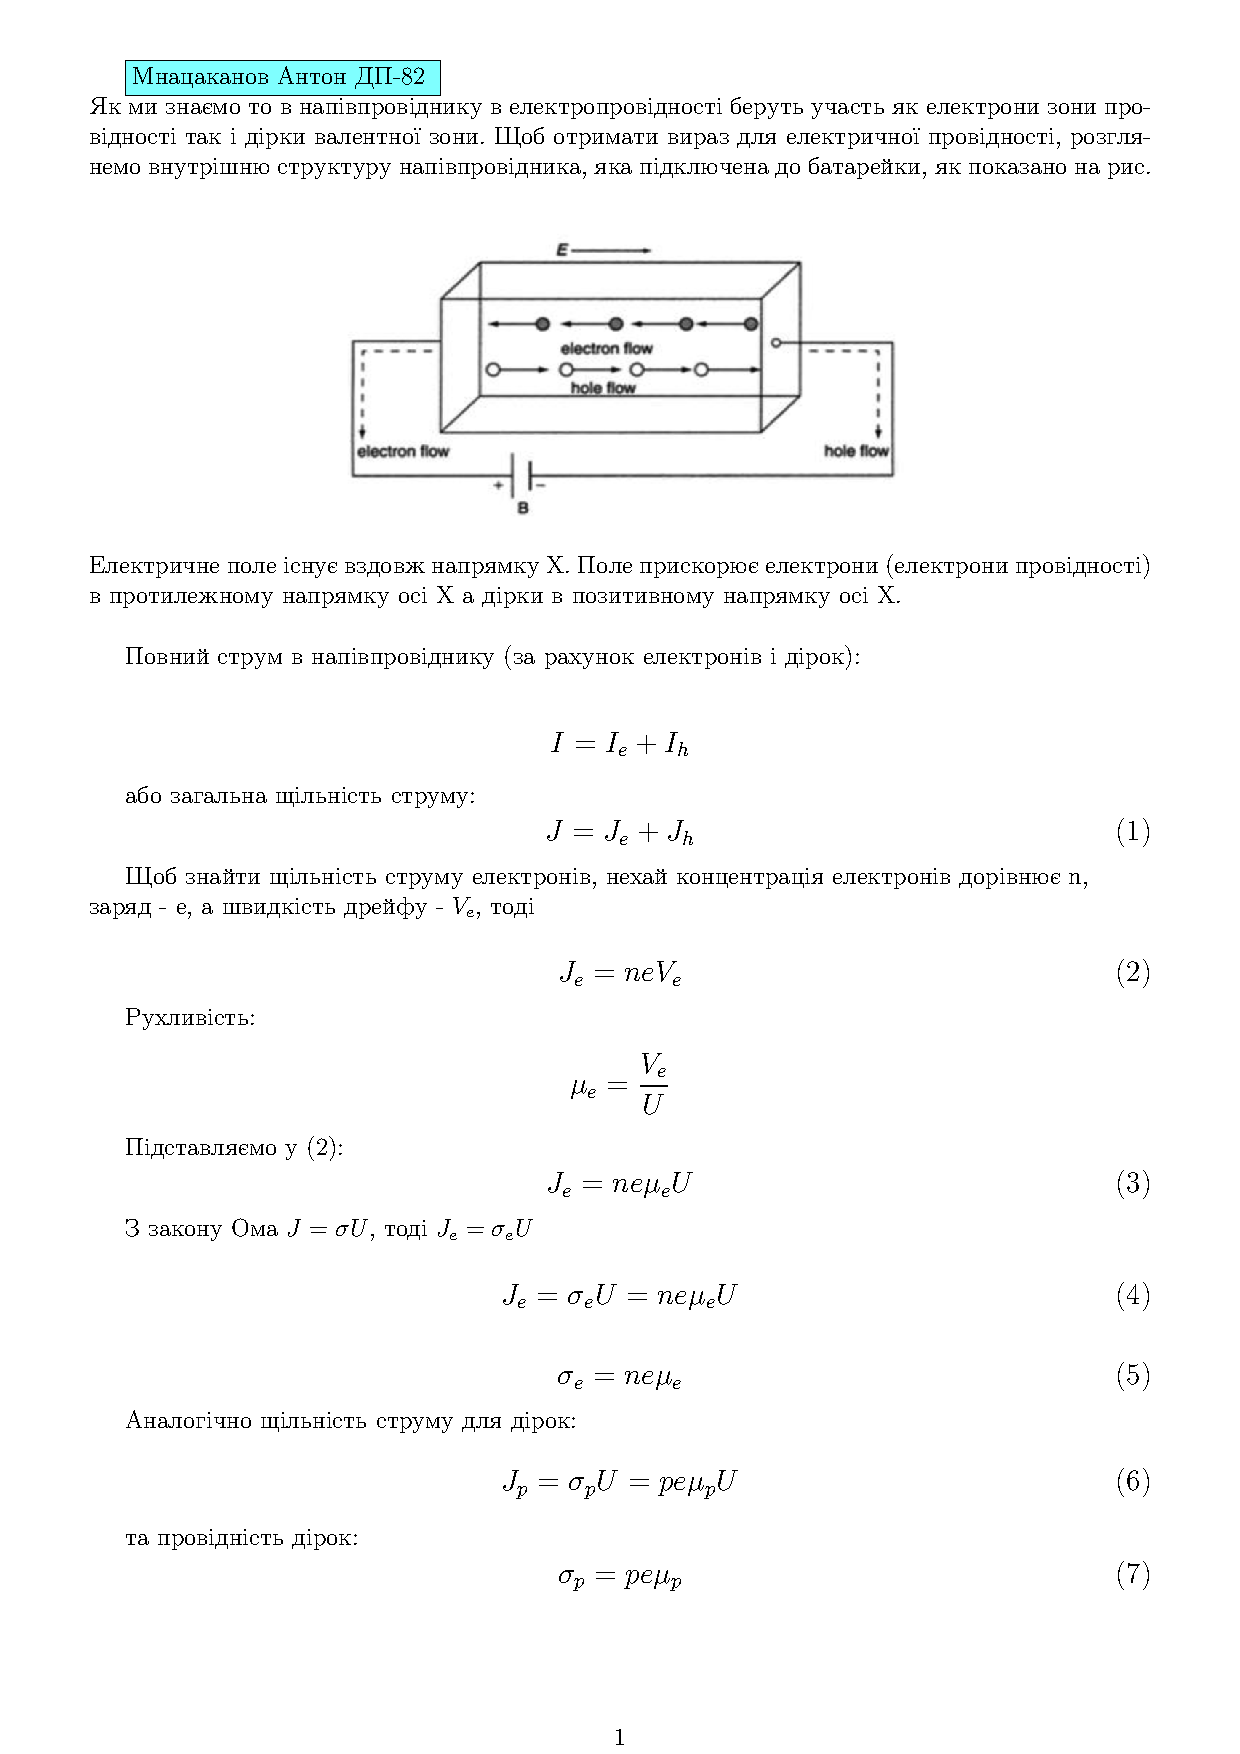
\includegraphics[scale=#3]{#1.#2}\label{#4}}
\end{figure}

}

\section*{\textrm{1. Мета роботи}}

Ознайомитися з принципом побудови і логікою роботи
ЦАП і АЦП, визначити основні параметри.

\section*{\textrm{2. Завдання}}



 Вивчити принцип дії, логіку роботи і параметри ЦАП, АЦП.\\

 Накреслити тимчасові діаграми ЦАП і АЦП, що пояснюють їх роботу.\\

 Дослідити принцип роботи цифро-аналогового перетворювача.\\

\begin{enumerate}
\item Встановити генератор в режим «Ручная синхронизация», вольтметр підключити до контрольної точки КТ4.
\item Перемикачі П1 і П2 стенда встановити в відключений стан (вимкнений).
\item Встановити нульовий стан лічильника шляхом короткочасного натискання перемикача П2.
\item Здійснити послідовний запуск генератора кнопкою ручної синхронізації.
При цьому після кожного натискання необхідно вимірювати вихідну напругу
(КТ4) за допомогою цифрового вольтметра. Результати вимірювань внести в
таблицю.
\item За результатами вимірювань виконати розрахунки диференціальної і
інтегральної нелінійності перетворювача.
\item Перевести схему ЦАП в циклічний режим шляхом перемикання
генератора Г5-54 в режим автоматичної синхронізації. Підключити замість
вольтметра осцилограф до контрольної точки КТ4 (синхронізація осцилографа
контрольною точкою КТ2). Замалювати вихідний сигнал ЦАП в контрольній
точці КТ4. Також замалювати в збільшеному масштабі вихідний сигнал ЦАП,
щоб було видно декілька перших сходинок.

\item За допомогою осцилографа визначити:
\begin{trivlist}
\item а) час встановлення першої сходинки вихідного сигналу ЦАП;
\item б) час обнулення ЦАП.
\end{trivlist}

\end{enumerate}

 Дослідити принцип роботи аналого-цифрового перетворювача.

\begin{enumerate}

\item Переключити стенд в режим АЦП. Для цього натиснути перемикач П1, а перемикач П2 має бути вимкнений.
\item Встановити частоту генератора $f = 22$ кГц і тривалість імпульсу $t_i = 20$ мкс.
\item Підключити вольтметр до контрольної точки КТ1.
\item За допомогою регулювання «$U_{\text{вх}}$, В» на стенді послідовно встановлювати напругу від 0 до 3,5 В з кроком 0,5 В.
\item Результати вимірювань записати в таблицю і побудувати графік чисельного значення коду від вхідної напруги.
\item Визначити інтегральну і максимальну диф-ну нелінійність перетворення.
\item Встановити $U_{\text{вх}} = 3,6$ В. Синхронізувати осцилограф контрольною
точкою КТ2. Зняти і побудувати часові діаграми роботи АЦП (контрольні
точки КТ2, КТ3, КТ4). Виміряти час встановлення вихідного коду.

\end{enumerate}




\section*{\textrm{3. Схема вимірювання}}

%\print{adc_dac}{png}{0.7}{}{Схема дослідження АЦП та ЦАП.}

\begin{figure}[h!]
  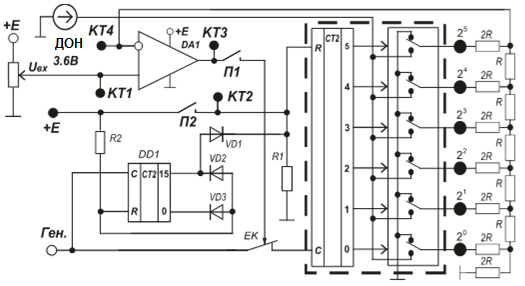
\includegraphics[width=0.55\linewidth]{adc_dac.png}
\end{figure}

\newpage
\section*{\textrm{4. Результати вимірювання}}


\begin{figure}[!h]\TopFloatBoxes\CenterFloatBoxes
\ttabbox[\FBwidth+5cm]{\caption{Залежність вихідної напруги ЦАП від числа вхідних імпульсів.}}
{
\begin{tabular}{|c|c|c|c|c|c|c|c|}
\hline
\begin{tabular}[c]{@{}c@{}}к-сть\\ імпульсів\end{tabular} & 0  & 10  & 20   & 30   & 40   & 50   & 60   \\ \hline
U, мВ                                                     & 40 & 640 & 1240 & 1840 & 2440 & 3040 & 3640 \\ \hline
\end{tabular}
}
\end{figure}


\print{dac_diag}{jpg}{0.4}{tsap}{Вихідний сигнал ЦАП.}

\newcommand{\RomanNumeralCaps}[1]
    {\MakeUppercase{\romannumeral #1}}


Час перемикання першої сходинки $t_{\text{вст.}\RomanNumeralCaps{1}}$ = 8,4 мкс. Час обнулення ЦАП становить 8 мкс.

\begin{figure}[!h]\TopFloatBoxes\CenterFloatBoxes
\ttabbox[\FBwidth+5cm]{\caption{Оцифровані величини вхідної напруги АЦП.}}
{
\begin{tabular}{|c|c|c|}
\hline
$U_{\text{вх}}$, В & Двійковий код АЦП & Десятковий код АЦП \\ \hline
0                  & 000001            & 1                  \\ \hline
0,5                & 001001            & 9                  \\ \hline
1                  & 010001            & 17                 \\ \hline
1,5                & 011001            & 25                 \\ \hline
2                  & 100010            & 34                 \\ \hline
2,5                & 101010            & 42                 \\ \hline
3                  & 110011            & 51                 \\ \hline
3,5                & 111011            & 59                 \\ \hline
\end{tabular}
}
\end{figure}

\newpage

\print{1111}{png}{0.5}{adc_time}{Графік чисельного значення коду від вхідної напруги.}

\print{adc_diag}{jpg}{0.5}{adc_time}{Часові діаграми роботи АЦП}


\newpage

\section*{\textrm{5. Висновок}}
  У ЦАП як видно з рис. 1,
вихiднi значення напруги зв’язанi з кiлькостю розрядiв ЦАП, выд яких і залежить крок збiльшення Uвих, а от  АЦП, Судячи з табл.2(Оцифрованi величини вхiдної напруги АЦП.), цей компонент працює зовсім навпаки, тобто він зчитує аналоговi величини та в подальшому оцифровує їх.

\clearpage
\section*{\textrm{6. Захист}}
1. Записати значення вихідної напруги Uвих ЦАП, якщо величина опорної
напруги Uо=3,6 В, а на вхід 5-розрядного ЦАП подано код 11010? (крайня
права 1 відповідає наймолодшому розряду). Записати формулу та
розрахунки.\\ 
\[ U_{\text{вих}}  = U_0\cdot(\dfrac{a_1}{2^1} + \dfrac{a_2}{2^2} +...+ \dfrac{a_n}{2^n}) \]

\begin{align*}
U_{\text{вих}}  = 3.6\cdot (\dfrac{1}{2}  +\dfrac{1}{4} +\dfrac{0}{8}  +\dfrac{1}{16}  +  0) = 2,925
\end{align*}

2. Якщо пронумерувати індикатори в схемі від 1 (найнижчий) до 6
(найвищий), а на вхід ЦАП подати код числа 25, то які з індикаторів будуть
світитися? \\
Будуть світитися:  1, 4 та 5 світлодіоди.\\

3. Призначення лічильника з 6-ма виходами в схемі.\\ 
Управляє ключами які підключають резисторами матриці RR-R2 до ДОН.\\ 

4. Чим обумовлено початок режиму зберігання роботи АЦП?\\ 
Якщо напруга на інвертуючому вході DA1 перевищить вхідну (неінвертуючий вхід), відбудеться перемикання компаратора і розмикання ключа ЕК. При цьому АЦП перейде в режим зберігання. \\ 

5. Перемикач П2 використовується для схеми ЦАП чи АЦП? Для чого саме
використовується?\\ 
Саме в мене Він призначений для того щоб обнуляти лічильник

 

\end{document}